\documentclass{article}

\usepackage{graphicx}
\usepackage{tikz}
\usepackage{tikzsymbols}
\usetikzlibrary{calc,patterns,shapes.geometric}
\pagestyle{empty}
\usepackage[margin=0pt]{geometry}
\geometry{papersize={14in,12in}}

\def\centerarc[#1](#2)(#3:#4:#5){\draw[#1] ($(#2)+({#5*cos(#3)},{#5*sin(#3)})$) arc (#3:#4:#5);}

\begin{document}
	\begin{figure}
		\centering
		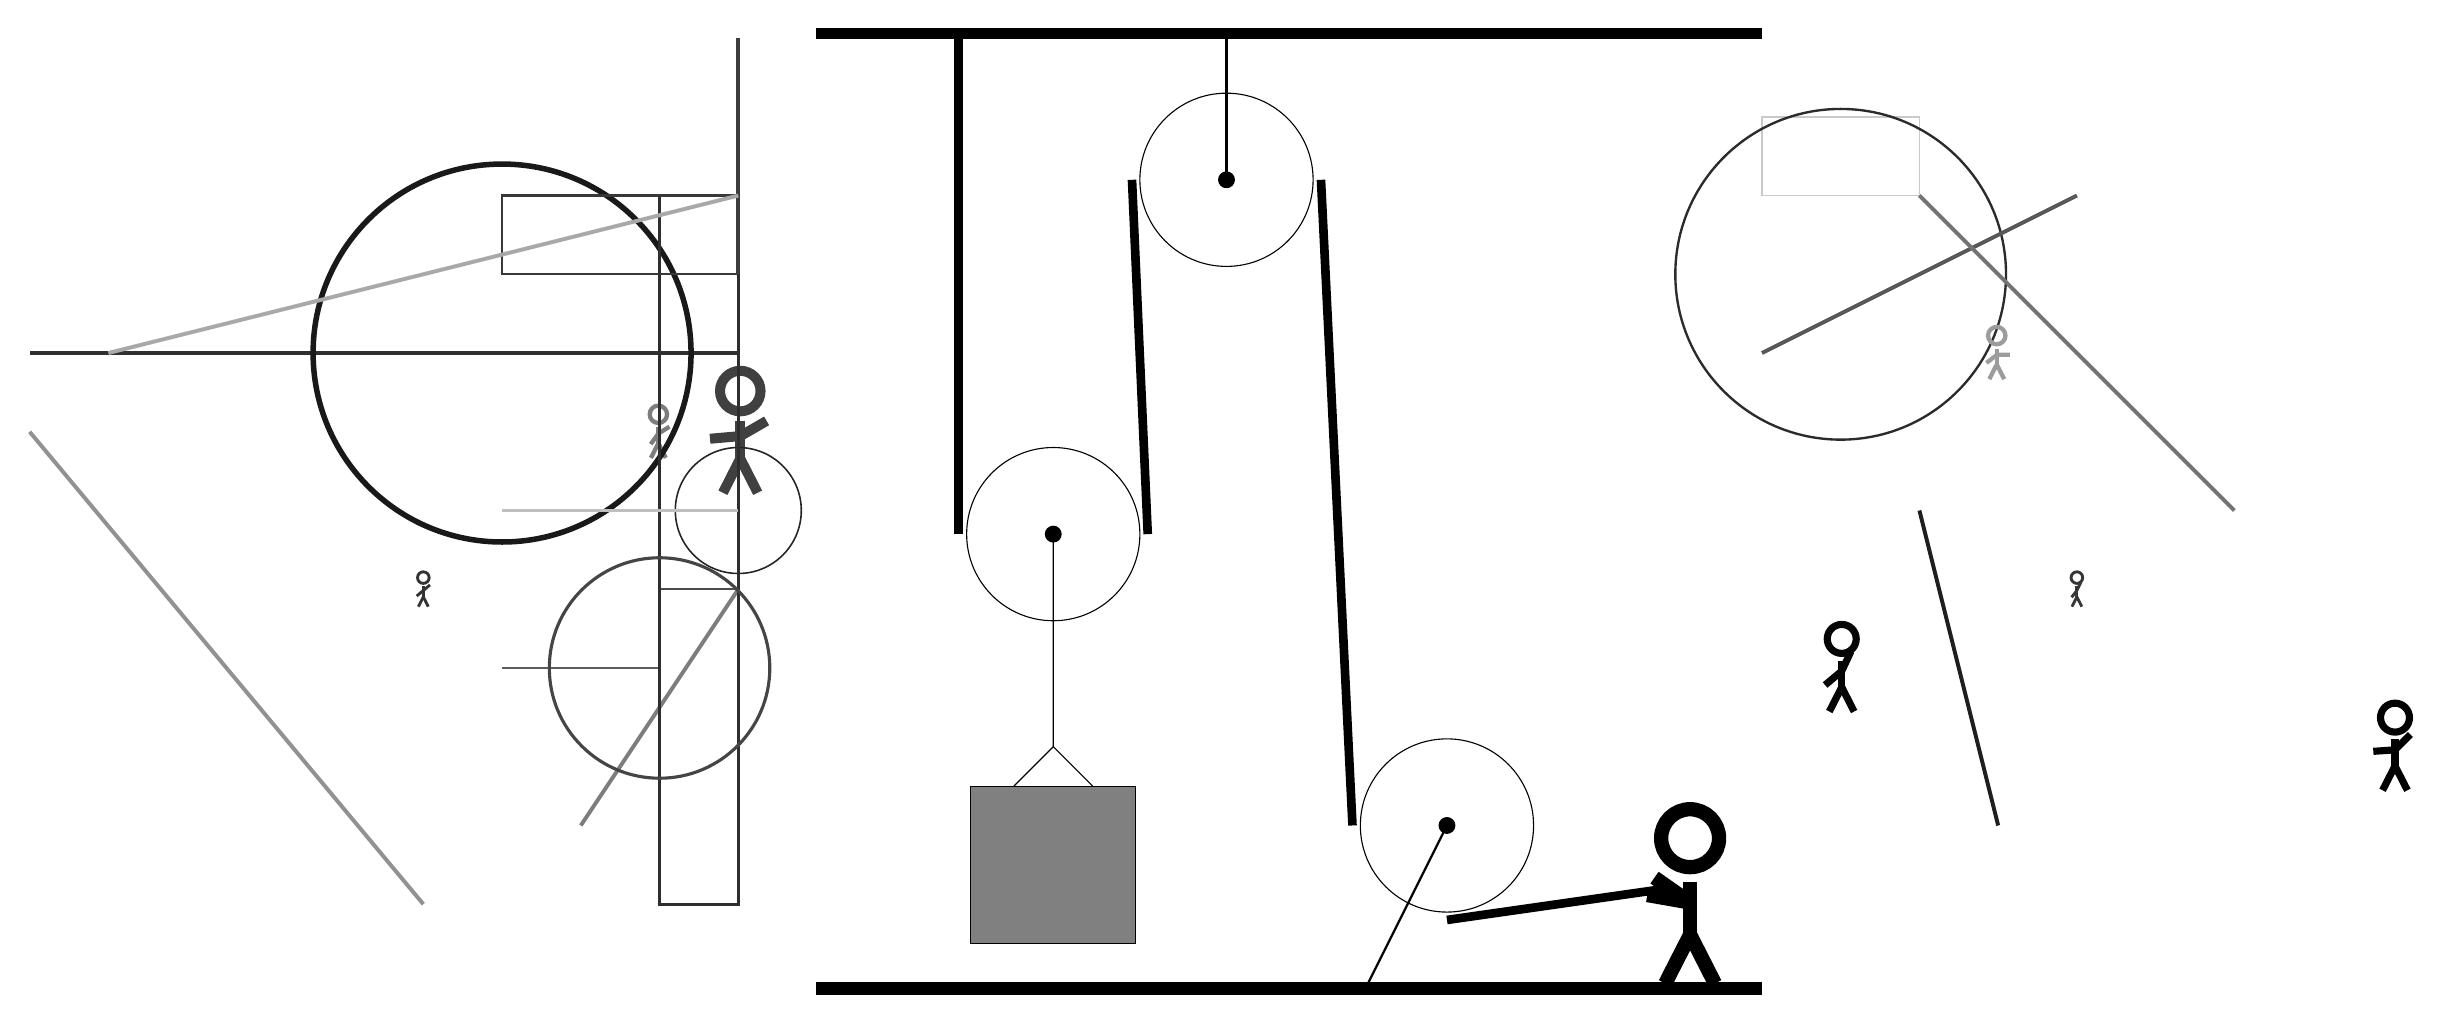
\begin{tikzpicture}
			%%%%% START %%%%%
			
			\draw[fill=black] (-2, 9) rectangle (10, 9.125);
			
			\draw (3.2, 7.2) circle (1.1);
			\draw[fill=black] (3.2, 7.2) circle (0.1);
			\draw[thick] (3.2, 7.2) -- (3.2, 9);
			
			\draw[line width=0.2mm, color=black!70] (-3, 6) rectangle (-4, 2);
			
			\node[line width=0.6mm, color=black!51] at (-4, 4) {\Strichmaxerl[3][54][32]};
			\draw[line width=0.5mm, color=black!81](-3, 5) -- (-12, 5);
			\node[line width=0.7mm, color=black!75] at (-3, 4) {\Strichmaxerl[7][5][30]};
			\draw [line width=0.2mm, color=black!86](-3, 3) circle (0.8);
			\draw[line width=0.3mm, color=black!64] (-4, 1) rectangle (-6, 1);
			\draw[line width=0.2mm, color=black!21] (10, 7) rectangle (12, 8);
			\draw [line width=0.3mm, color=black!83](11, 6) circle (2.1);
			\draw [line width=0.7mm, color=black!90](-6, 5) circle (2.4);
			\draw[line width=0.5mm, color=black!51](-3, 2) -- (-5, -1);
			\draw[line width=0.4mm, color=black!82] (-3, 7) rectangle (-4, -2);
			
			\draw[line width=0.5mm, color=black!65](14, 7) -- (10, 5);
			\draw[line width=0.3mm, color=black!78] (-3, 7) rectangle (-6, 6);
			
			\node[line width=0.3mm, color=black!100] at (18, 0) {\Strichmaxerl[5][4][45]};
			\draw[line width=0.5mm, color=black!88](13, -1) -- (12, 3);
			\draw [line width=0.4mm, color=black!73](-4, 1) circle (1.4);
			
			\node[line width=0.5mm, color=black!80] at (-7, 2) {\Strichmaxerl[2][40][40]};
			\draw[line width=0.5mm, color=black!43](-7, -2) -- (-12, 4);
			\draw[line width=0.5mm, color=black!55](12, 7) -- (16, 3);
			\node[line width=0.6mm, color=black!39] at (13, 5) {\Strichmaxerl[3][38][1]};
			\draw[line width=0.5mm, color=black!25](-6, 3) -- (-3, 3);
			
			\draw[line width=0.5mm, color=black!76](-3, 9) -- (-3, 6);
			\draw[line width=0.5mm, color=black!34](-3, 7) -- (-11, 5);
			\node[line width=0.4mm, color=black!79] at (14, 2) {\Strichmaxerl[2][52][64]};
			\node[line width=0.6mm, color=black!98] at (11, 1) {\Strichmaxerl[5][40][65]};
			
			
			\draw (6, -1) circle (1.1);
			\draw[fill=black] (6, -1) circle (0.1);
			\draw[thick] (6, -1) -- (5, -3);
			
			\draw (1, 2.7) circle (1.1);
			\draw[fill=black] (1, 2.7) circle (0.1);
			
			\draw (1, 2.7) -- (1, 0) -- (0.5, -0.5);
			\draw (1, 0) -- (1.5, -0.5);
			\draw[fill=black!50] (-0.05, -0.5) rectangle (2.05, -2.5);
			
			\draw[line width=1.1mm] (-0.2, 9) -- (-0.2, 2.7);
			\centerarc[line width=1.1mm](1, 2.7)(180:360:1.2000000000000002);
			\draw[line width=1.1mm](2.2, 2.7) -- (2.0, 7.2);
			\centerarc[line width=1.1mm](3.2, 7.2)(0:180:1.2000000000000002);
			\draw[line width=1.1mm](4.4, 7.2) -- (4.8, -1);
			\centerarc[line width=1.1mm](6, -1)(180:270:1.2000000000000002);
			\draw[line width=1.1mm](6, -2.2) -- (8.8, -1.8);
			
			\node at (9, -1.9) {\Strichmaxerl[10][-35][170]};
			
			\draw[fill=black] (-2, -3) rectangle (10, -3.15);
			
			%%%%% END %%%%%
		\end{tikzpicture}
	\end{figure}	
\end{document}